\documentclass[xcolor=svgnames]{beamer}
\mode<presentation>
{
      \setbeamertemplate{footline}[page number]
      \setbeamercovered{transparent}
      \setbeamertemplate{navigation symbols}{}
      \usecolortheme[named=DarkGreen]{structure}
}

\usepackage[english]{babel}
\usepackage{times}
\usepackage{url}
\usepackage{CJKutf8}
\usepackage{graphics}
\usepackage{amsmath}

\begin{document}
\begin{CJK*}{UTF8}{gbsn}


\title{内存管理}

%\begin{frame}
%\maketitle
%\end{frame}

\begin{frame}{第6次编程作业:寻找互素数对}
%\maketitle
\begin{equation}
4 \perp 9, \quad 34 \perp 35
\end{equation}

\begin{equation}
\Pr(m \perp n) = \frac{6}{\pi^2} \approx 0.607927102
\end{equation}

\end{frame}

\begin{frame}{第6次编程作业:寻找互素数对}
%在Intel Core2 Duo上,计算100000以内(共100亿个数对)互素的数对个数,
%结果是6079301507(理论预测值为6079271020,误差万分之0.05), 用时18分钟。
\begin{itemize}
\item 硬件平台:Intel Core2 (Duo)
\item 计算100000以内互素的数对的个数
\item 共涉及100亿个数对
\item 计算结果:6079301507
\item 理论预测:6079271020
\item 相对误差:万分之0.05
\item 耗时:18分钟
\item 本次作业:用多线程编程技术加速
\end{itemize}
\end{frame}

\begin{frame}{第6次编程作业--要求}
\begin{enumerate}
\item 输出结果:必须与单线程结果(6079301507)保持一致
\item 电子邮件发送内容
\begin{itemize}
\item 源程序
\item 文档:描述软硬件平台,记录原始testgcd.c运行时间,2-10个线程加速后运行时间,你们的分析
\end{itemize}
\item 手写报告内容
\begin{itemize}
\item 每位队员的贡献(简短描述)
\item 全体队员签名
\end{itemize}
\end{enumerate}
\end{frame}

\begin{frame}{推荐阅读文章}
\begin{enumerate}
\item 如何成为一名黑客 (作者: Eric S. Raymond, 英文How to become a hacker)
\item 完全用Linux工作  (作业:王垠)
\end{enumerate}
\end{frame}

\begin{frame}{Parkinson's law}
\begin{columns}%[t]
\column{.5\textwidth}
\begin{enumerate}
\item Work expands so as to fill the time available for its completion.
\item[]
\item Data expands to fill the space available for storage.
\end{enumerate}
\column{.5\textwidth}
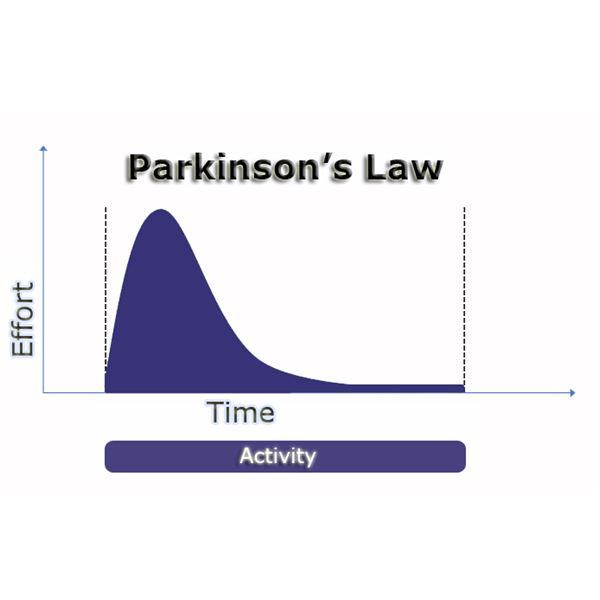
\includegraphics[width=1.0\textwidth]{parkinson.jpg}
\end{columns}%[t]
\end{frame}

\begin{frame}{程序员希望的内存}
\begin{columns}%[t]
\column{.5\textwidth}
\begin{block}{联系上次作业}
私有的、无穷大、无穷快、便宜、持久性
\end{block}
\column{.5\textwidth}
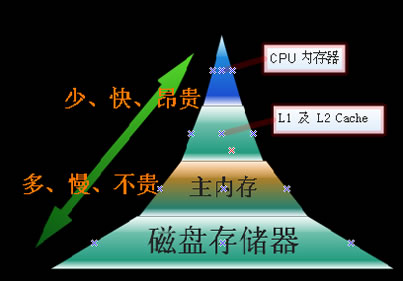
\includegraphics[width=1.0\textwidth]{memory_hier.jpg}
\end{columns}%[t]
\end{frame}

\begin{frame}{内存管理器(Memory Manager)的任务}
\begin{itemize}
\item 提供内存抽象界面
\item 分配物理内存,回收物理内存
\item 记录内存使用情况等
\end{itemize}
\end{frame}

\begin{frame}{没有内存抽象:程序员直接操作物理内存}
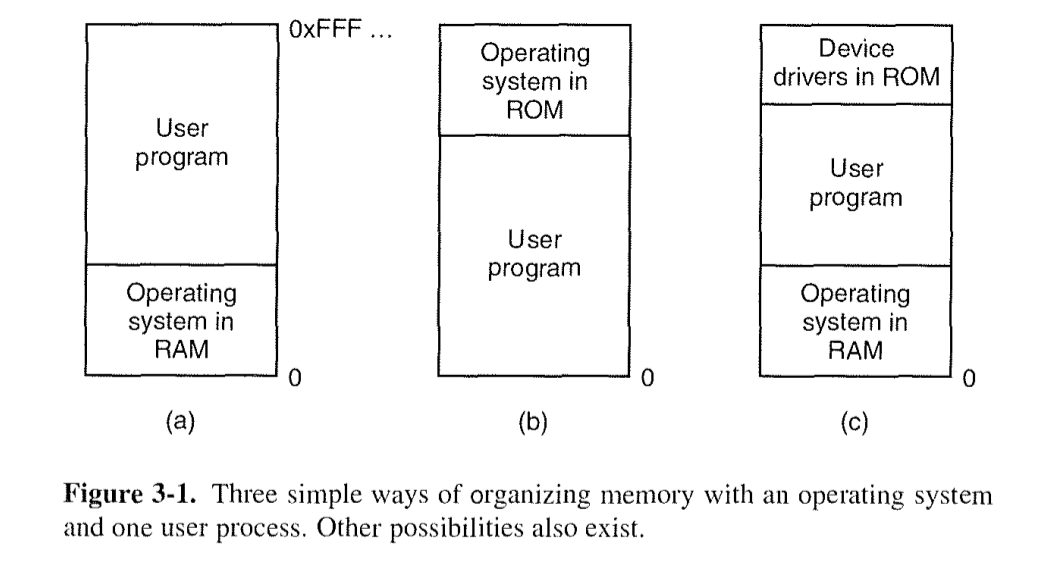
\includegraphics[width=1.0\textwidth]{nomem.png}

a. 内存中一次只能驻留一个程序:\alert{MOV REGISTER1, 1000}

b. 操作系统自身代码难以保护(没有地址空间概念)
\end{frame}

\begin{frame}{虚拟内存技术}
%虚拟内存技术可解决个问题:
\begin{itemize}
\item 问题一:如何让多个程序驻留内存?
\begin{itemize}
\item 每个程序有专属地址空间
\item 程序不能非法访问其他程序的地址空间
\end{itemize}
\item 问题二:如何满足程序对内存的无限需求?
\begin{itemize}
\item 地址空间分成若干\alert{页面}
\item 地址空间的页面映射到物理内存的\alert{页框}内
\item 利用\alert{页表}实现页面号到页框号的映射
\item 不是所有的页面都需要放到物理内存中
\item 缺页中断技术
\end{itemize}
\end{itemize}
\end{frame}

\begin{frame}{虚拟内存技术}
分页技术的精髓:不是所有页面都需要同时调入内存
\end{frame}

\begin{frame}{虚拟地址、物理地址及内存管理单元}
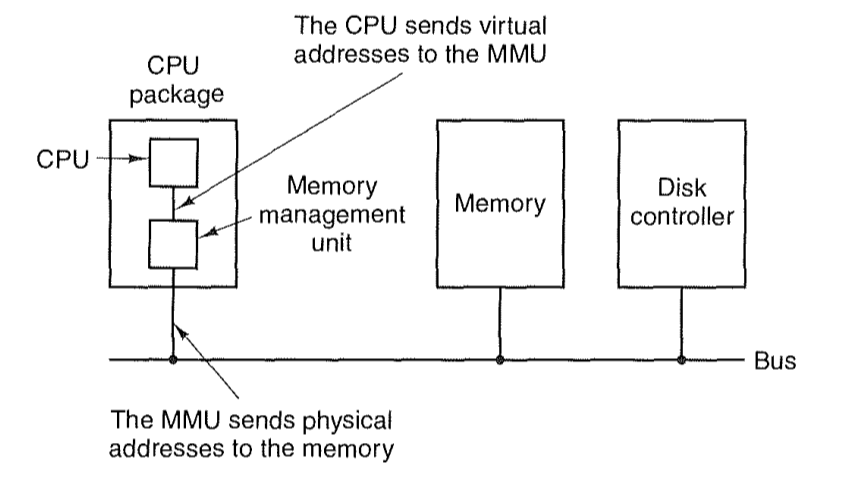
\includegraphics[width=0.9\textwidth]{mmu.png}

\alert{注意}:程序中的地址全都是虚拟地址
\end{frame}

%\begin{frame}{系统调用的例子}
%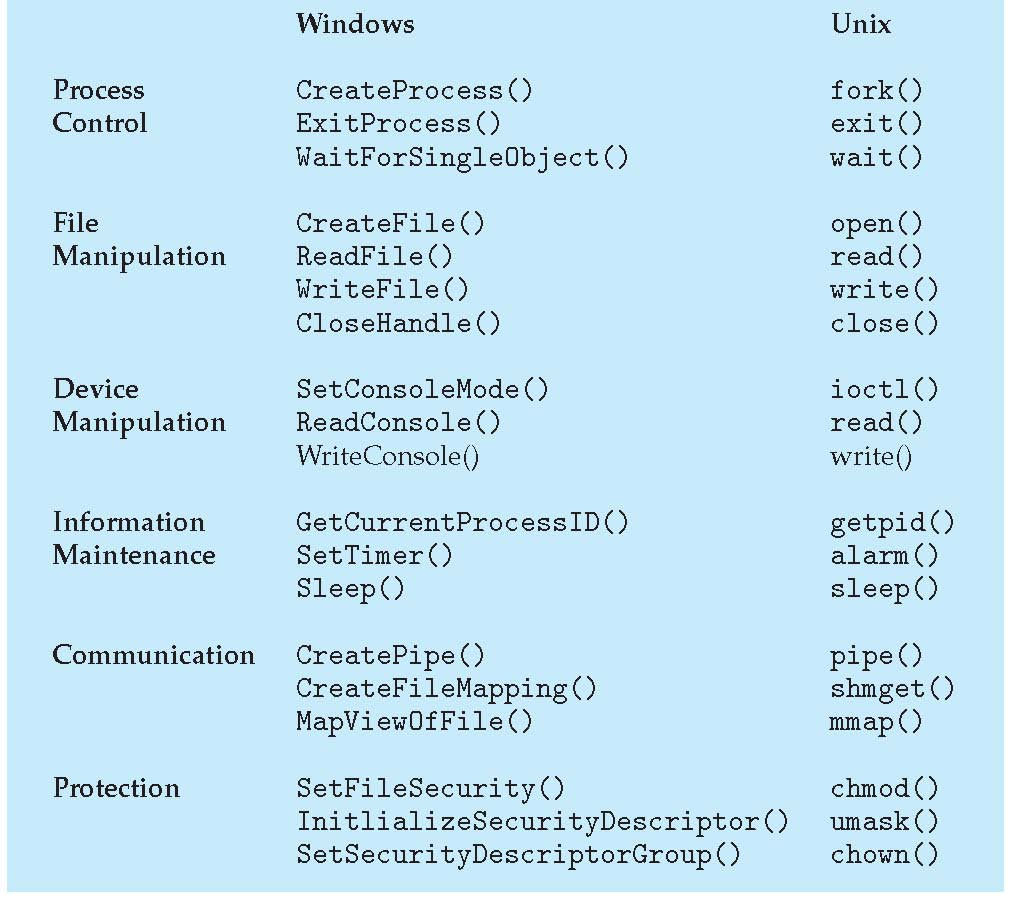
\includegraphics[width=0.9\textwidth]{examples.jpg}
%\end{frame}

\begin{frame}{虚拟地址、物理地址及内存管理单元}
\begin{columns}%[t]
\column{.4\textwidth}
\begin{itemize}
\item 虚拟地址空间:64K (16 bit)
\item 物理地址空间:32K (15 bit)
\item 页面大小:4K 
\item 共16个(虚拟)页面,8个(物理)页框
\item 对于大于32K的程序,只能有32K驻留物理内存(右图数字部分)
\end{itemize}
\column{.6\textwidth}
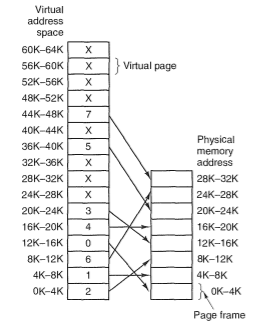
\includegraphics[width=1.0\textwidth]{vm.png}
\end{columns}%[t]
\end{frame}

\begin{frame}{虚拟地址、物理地址及内存管理单元}
\begin{columns}%[t]
\column{.4\textwidth}
\begin{block}{MOV REG, 20500}
20500 = 5 * 4K + 20 

页面5 $\rightarrow$ 页框3

12K + 20 = 12308(物理地址)
\end{block}
\begin{block}{MOV REG, 32780}
32780 = 8 * 4K + 12

对应虚拟页面8(缺页)

\alert{what next?}
\end{block}
\begin{block}{页表内容}
需要由操作系统维护
\end{block}
\column{.6\textwidth}
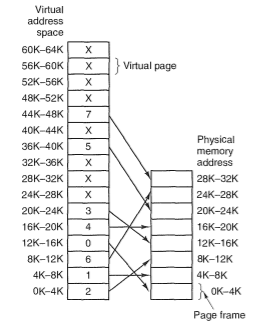
\includegraphics[width=1.0\textwidth]{vm.png}
\end{columns}%[t]
\end{frame}

\begin{frame}{虚拟地址、物理地址及内存管理单元}
\begin{columns}%[t]
\column{.4\textwidth}
虚拟地址映射到物理地址,考虑右图例子:
\begin{itemize}
\item 页面大小:4K 
\item 页内地址为12位
\item 对于16位机器而言,有4位用于页表索引
\item 因此共有16个虚拟页面
\item 8个物理页框(需3位)
\end{itemize}
\column{.6\textwidth}
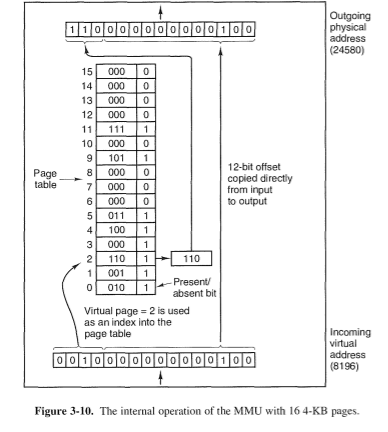
\includegraphics[width=1.0\textwidth]{mmu2.png}
\end{columns}%[t]
\end{frame}

\begin{frame}{页表项}
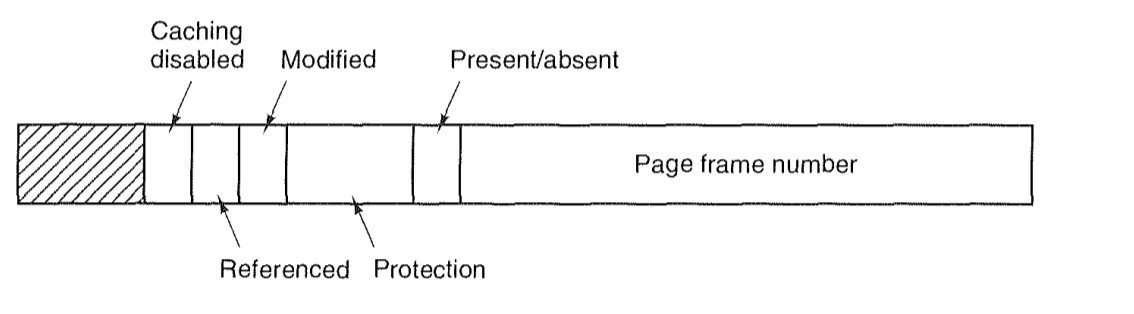
\includegraphics[width=1.0\textwidth]{pte.png}
\begin{description}
\item[page frame number]描述该页表项对应的页框编号
\item[present / absent]表示该页表是否在内存中
\item[protection]含读、写、执行等权限信息
\item[modified]该页表内容是否被修改过
\item[referenced]该页表内容是否被用过(读写)
\item[caching disabled]用于memory mapped I/O(后续)
\end{description}
\end{frame}

\begin{frame}{虚拟内存技术与分页技术面临的两大问题}
\begin{enumerate}
\item 从虚拟地址到物理地址的映射必须快
\begin{itemize}
\item 每条指令都需从内存取出
\item 大量指令涉及读写内存(CISC机器)
\end{itemize}
\item 如果虚拟地址空间很大,则页表规模会特别大

考虑页面大小4K的虚拟内存系统:
\begin{itemize}
\item 32位虚拟地址: 100万个页表项
\item 64位虚拟地址:45035996亿个页表项
\item 注意:每个进程都需要单独的页表!!
\end{itemize}
\end{enumerate}
\end{frame}

\begin{frame}{从虚拟地址到物理地址的快速映射:TLB(联想式存储)}
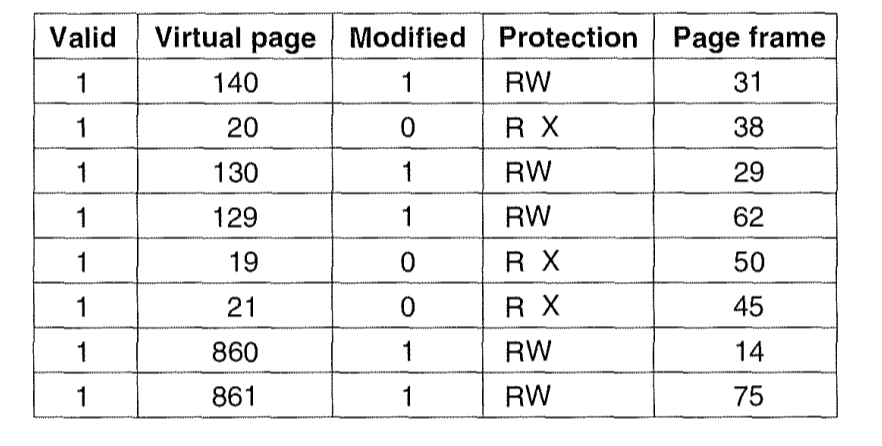
\includegraphics[width=1.0\textwidth]{tlb.png}

放置在MMU里面。来虚拟地址,先查TLB。
\begin{itemize}
\item 若能在TLB中查到该虚拟地址,则直接输出物理页框号码
\item 否则,去内存中的页表中查找对应页框号码,并将其调入TLB
\end{itemize}
\end{frame}

\begin{frame}{处理大规模地址空间的方法一:多级页表}
%\begin{columns}%[t]
%\column{.3\textwidth}
%多级页表:页表的全部内容不必都放在内存中
%\column{.7\textwidth}
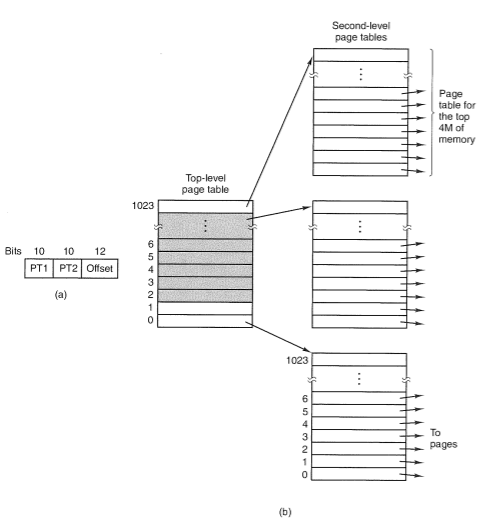
\includegraphics[width=0.7\textwidth]{multi.png}
%\end{columns}%[t]

多级页表:页表的全部内容不必都放在内存中
\end{frame}

\begin{frame}{处理大规模地址空间的方法二:倒排页表}
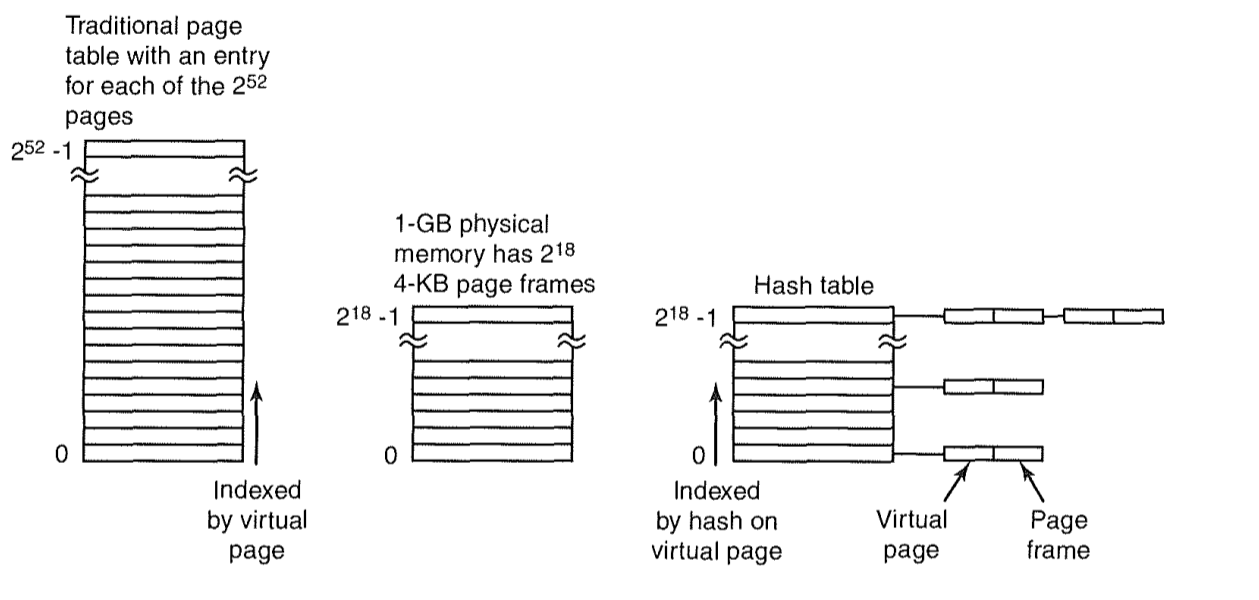
\includegraphics[width=1.0\textwidth]{inverted.png}
\end{frame}

\begin{frame}{页面置换算法}
当发生缺页时,OS需要选择一个页面将其从物理内存转移至硬盘,然后从硬盘调入所缺页面。
\end{frame}

\begin{frame}{老化(aging)页面置换算法}
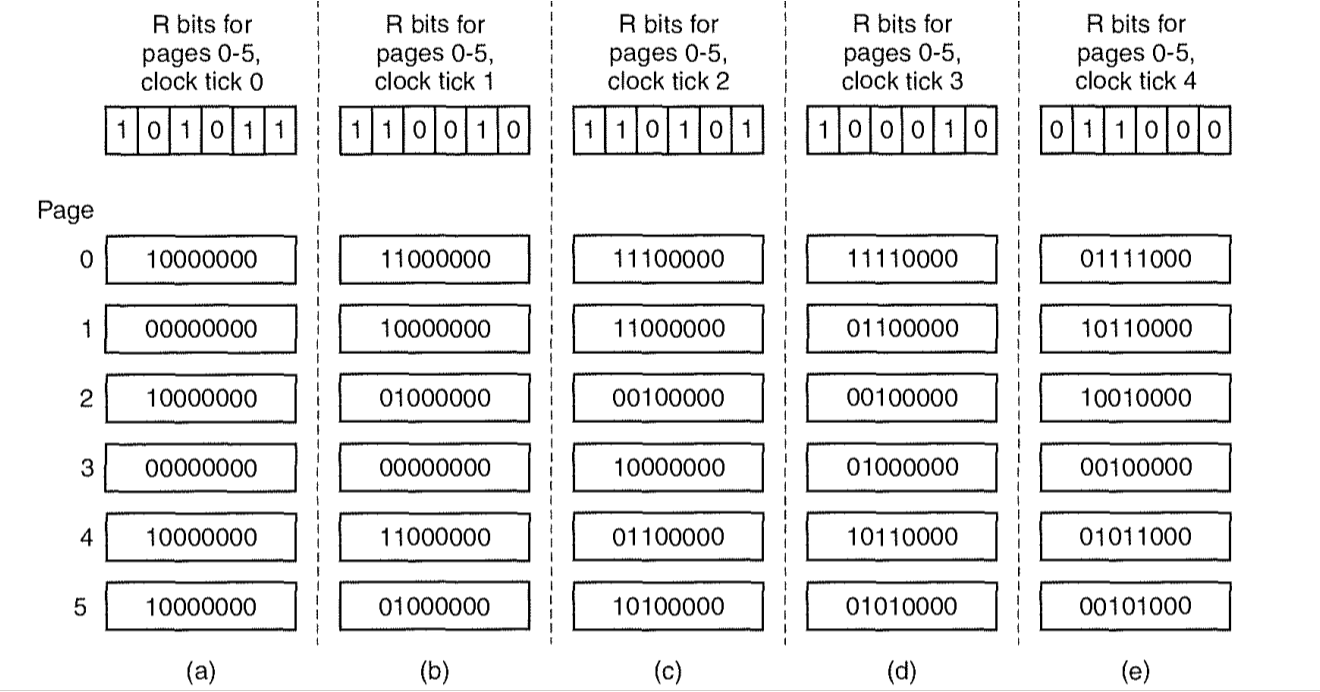
\includegraphics[width=1.0\textwidth]{aging.png}
\end{frame}

\begin{frame}{工作集(working set)页面置换算法}
\begin{itemize}
\item 访问的\alert{局部性}:在任一时间段内,程序仅仅访问其所有页面的一小部分。
\item[]
\item 我们将程序在某时间段内密集访问的页面集合成为\alert{工作集}
\end{itemize}
\end{frame}

\begin{frame}{工作集(working set)页面置换算法}
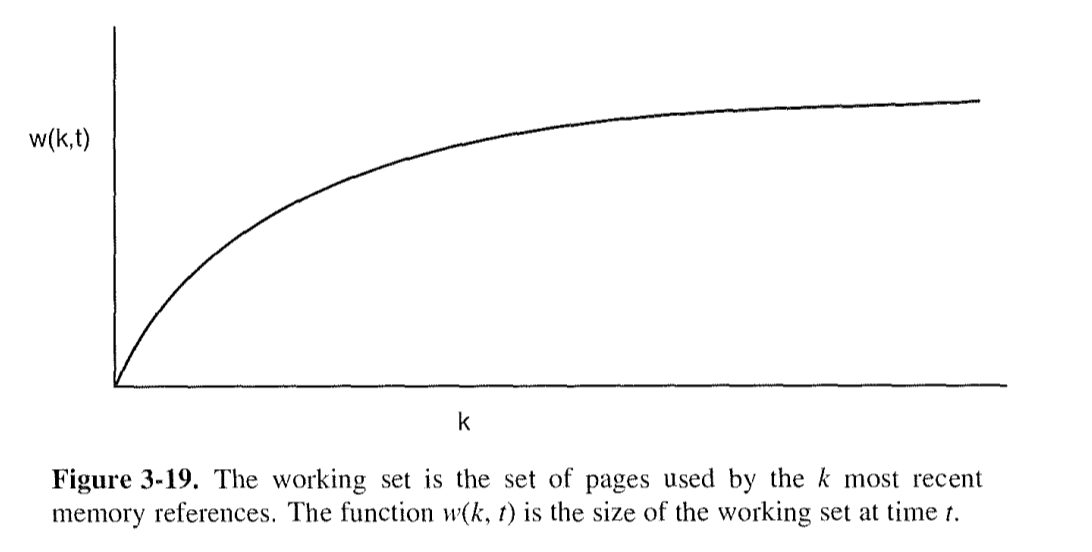
\includegraphics[width=1.0\textwidth]{ws0.png}
\end{frame}

\begin{frame}{工作集(working set)页面置换算法}
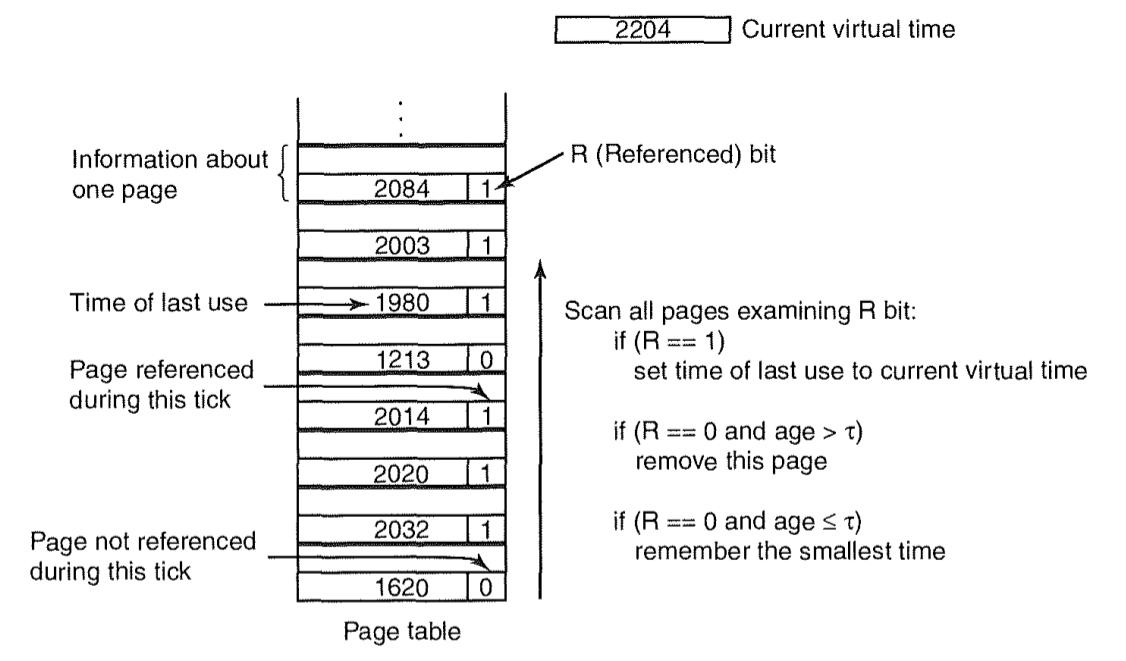
\includegraphics[width=1.0\textwidth]{ws.png}

思考:如果找不到不在工作集的页面,怎么办?
\end{frame}

\begin{frame}{WSClock页面置换算法}
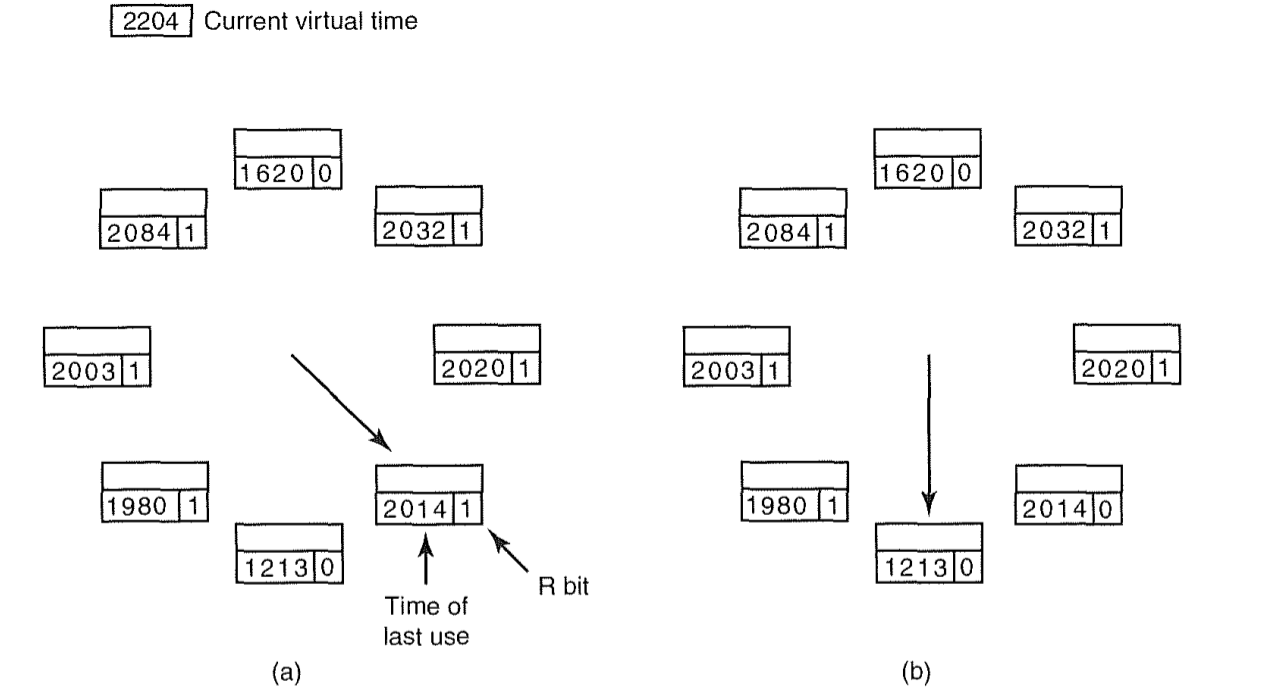
\includegraphics[width=1.0\textwidth]{wsclock1.png}

如果当前页R=1,将其设为0,然后考察下一页
\end{frame}

\begin{frame}{WSClock页面置换算法}
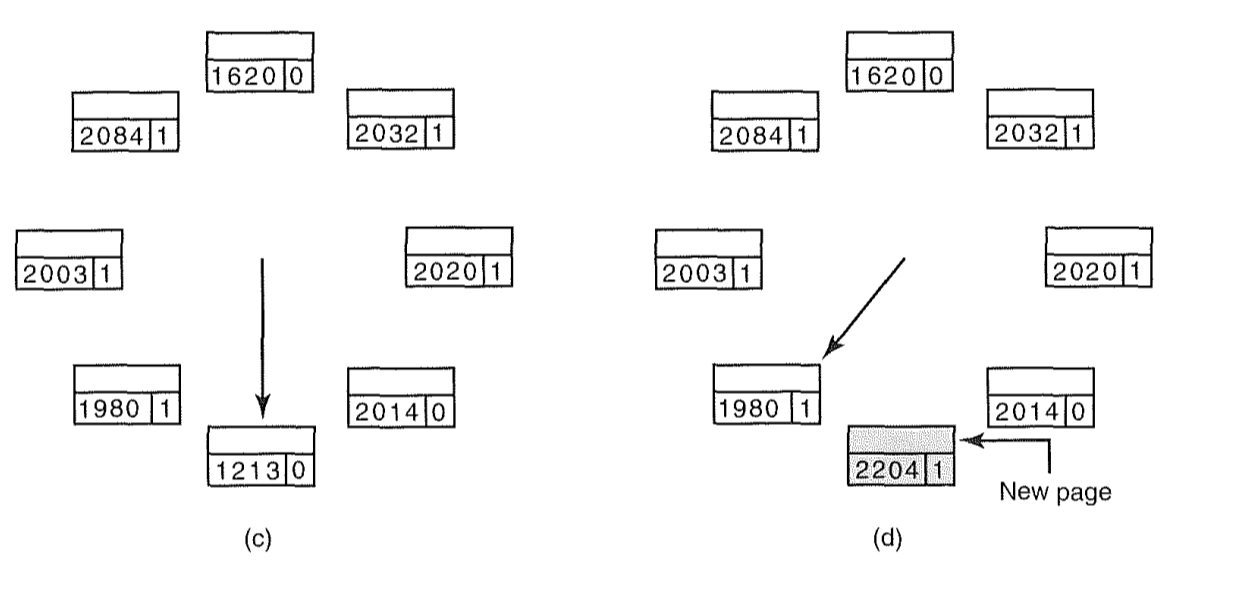
\includegraphics[width=1.0\textwidth]{wsclock2.png}

如果当前页R=0, M=0, 且其age足够大,则将其置换出物理内存% $设为0,然后考察下一页

思考:如果M不为0?
\end{frame}

\begin{frame}{分页技术:页面大小如何确定?}
%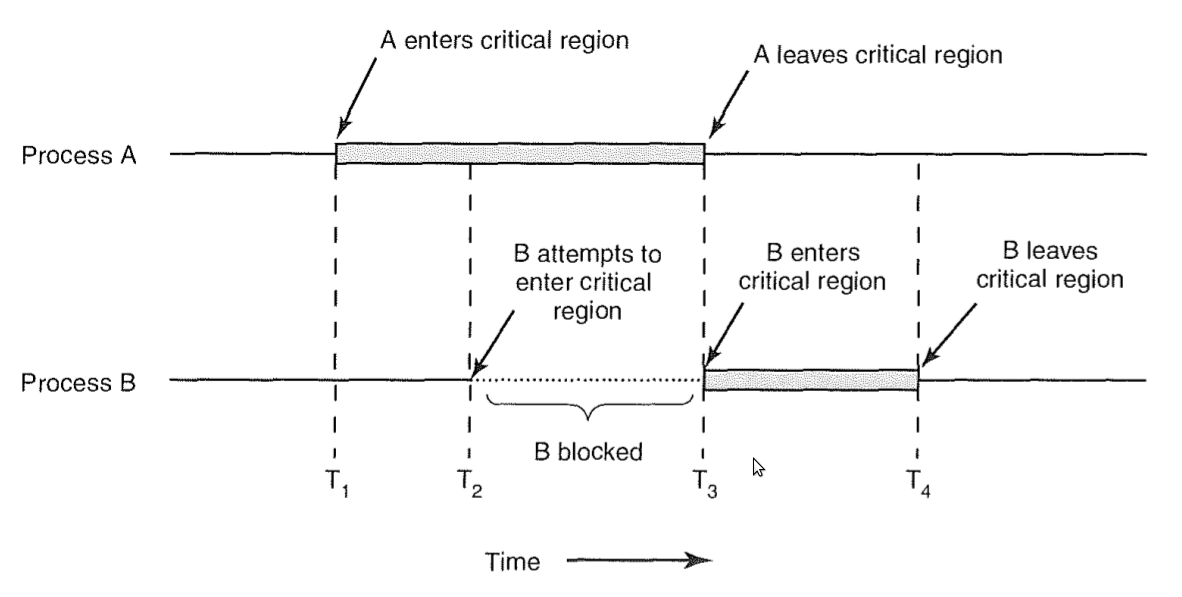
\includegraphics[width=1.0\textwidth]{mutual.png}
有以下几点考虑:
\begin{enumerate}
\item 页面太大?导致最后一页浪费太多(半页)
\item 页面太小,导致页表规模很大
\item 额外开销计算
\begin{equation*}
overhead = e \cdot \frac{s}{p} + \frac{p}{2}
\end{equation*}
其中,$p$为页面大小,s为进程平均大小(字节),e为每个页表项的大小(字节)
\end{enumerate}
容易算出,当$p = \sqrt{2s\cdot e}$时,额外开销最少
\end{frame}

\begin{frame}{单纯分页技术的缺点--分段技术的引入}
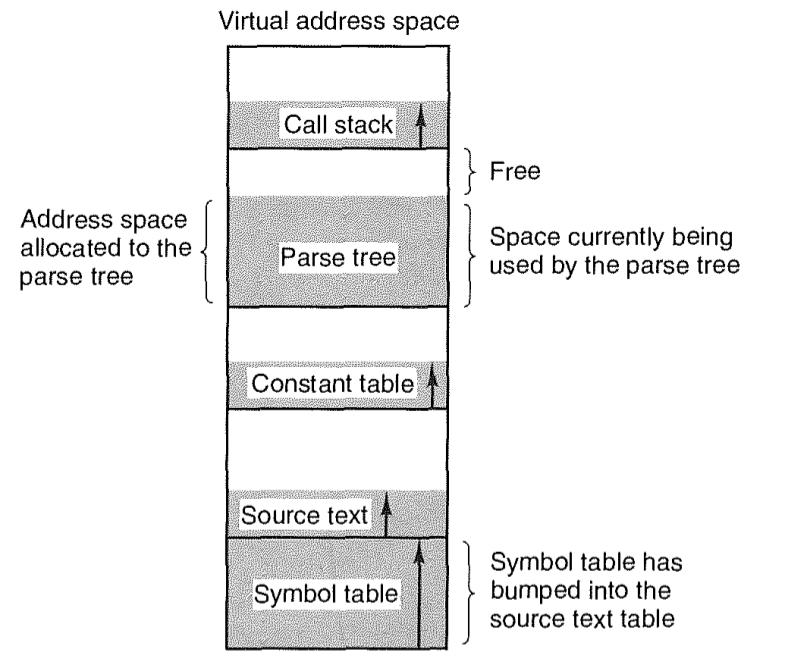
\includegraphics[width=0.7\textwidth]{noseg.png}
\end{frame}

\begin{frame}{单纯分页技术的缺点--分段技术的引入}
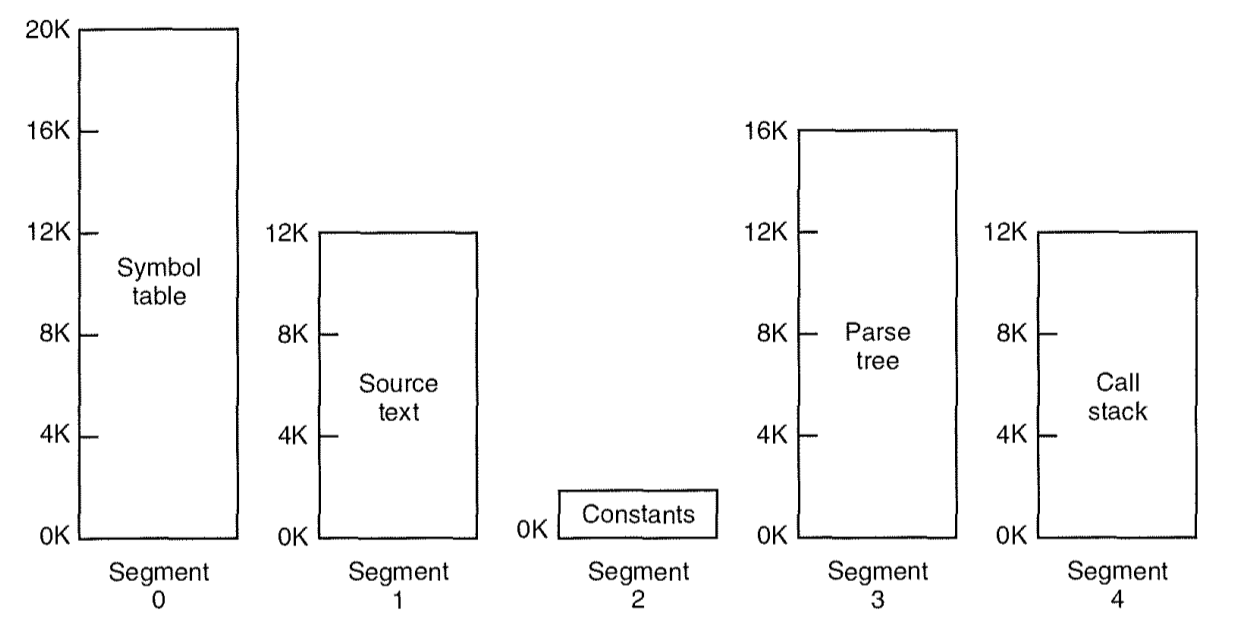
\includegraphics[width=1.0\textwidth]{seg.png}

每个段(segment)是独立的地址空间,互不干涉,可自如伸缩
\end{frame}

\begin{frame}{分段技术}
\begin{itemize}
\item 程序员(编译器)可见
\item 每个段可以对应子函数、栈、数组、其它类型变量中的一种(但一般不是多种)
\item 分段以后,更有利于保护(代码段--执行、数据段--读写)
\item 分段以后,更便于在进程间共享代码与数据
\end{itemize}
\end{frame}

\begin{frame}{分段与分页技术的比较}
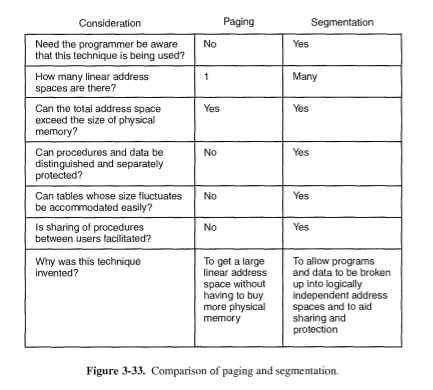
\includegraphics[width=1.0\textwidth]{comp.png}
\end{frame}

\begin{frame}{分段与分页技术相结合 --- 融合二者优点}
如果某个段(segment)特别大,无法全放入内存,怎么办?

\alert{答案}:针对每个段,采用分页技术。即只把每段中部分页面放入物理内存
\end{frame}

\begin{frame}{MULTICS的分段分页技术: 段表与页表}
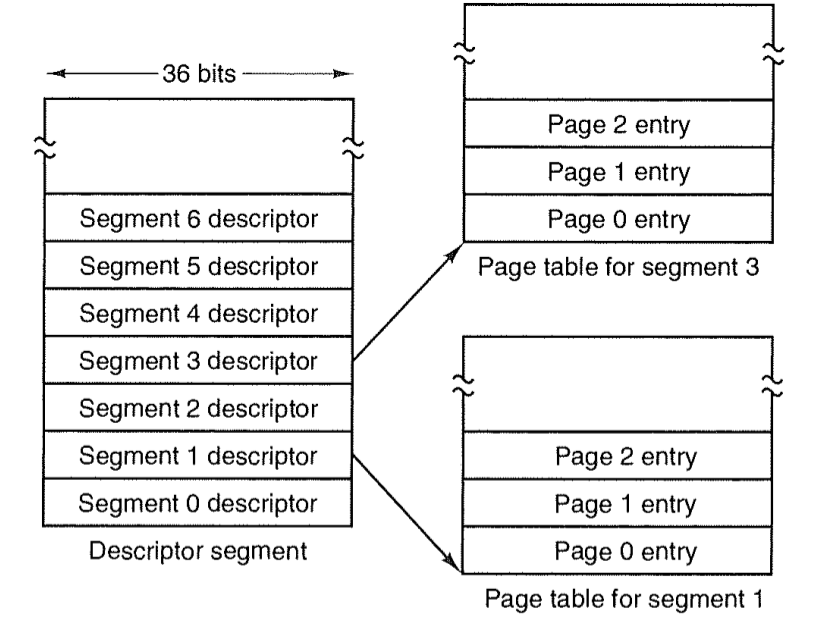
\includegraphics[width=1.0\textwidth]{seg1.png}
\end{frame}

\begin{frame}{MULTICS的分段分页技术: 段表项}
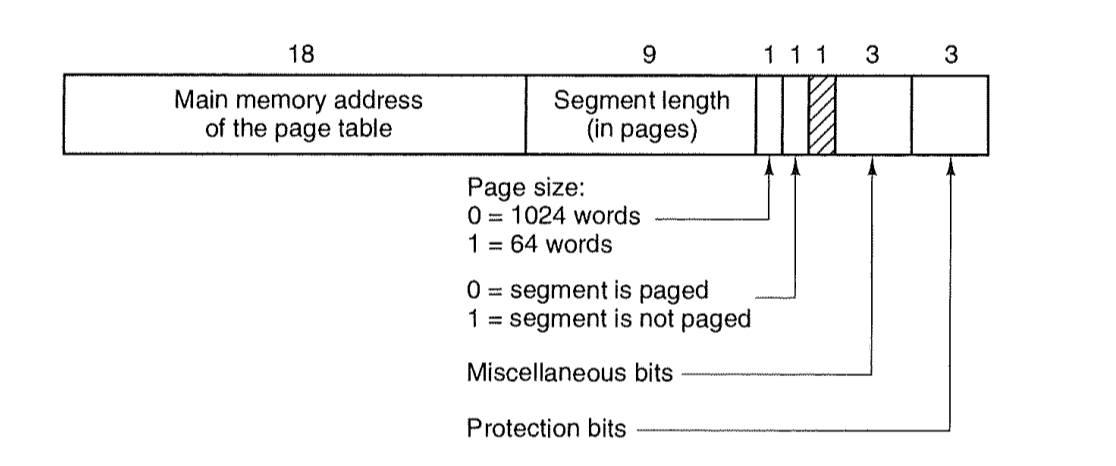
\includegraphics[width=1.0\textwidth]{seg2.png}
\end{frame}

\begin{frame}{MULTICS的分段分页技术: 虚拟地址格式}
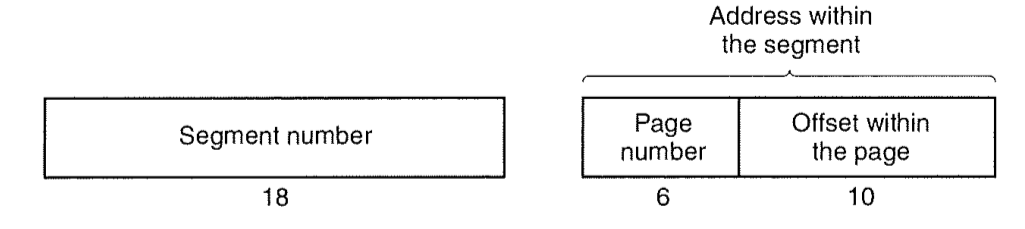
\includegraphics[width=1.0\textwidth]{seg3.png}

思考:MULTICS可以支持多少个段?%页面大小?页面个数?
\end{frame}

\begin{frame}{MULTICS的分段分页技术: 虚拟地址到物理地址的映射}
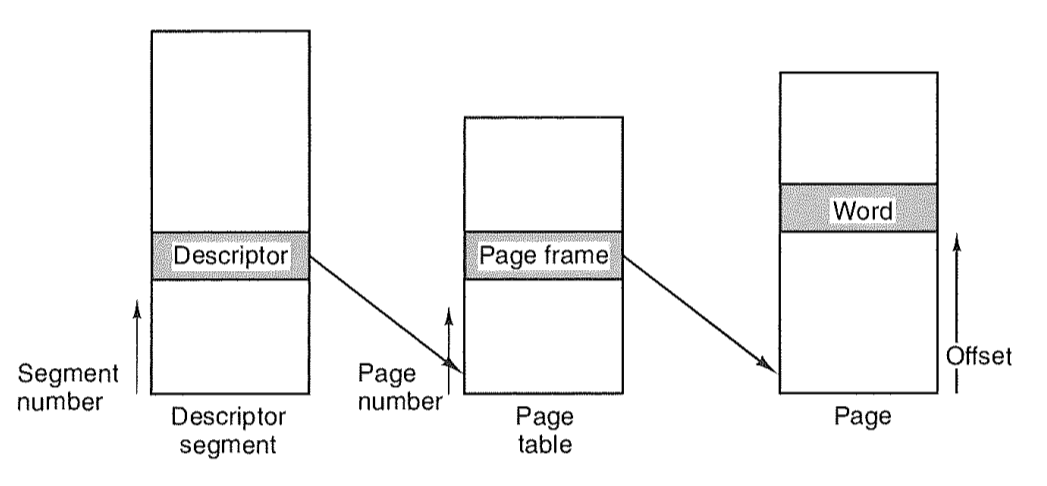
\includegraphics[width=1.0\textwidth]{seg4.png}
\end{frame}

\begin{frame}{MULTICS的分段分页技术: 虚拟地址到物理地址的映射}
\alert{问题:}如果每次访问内存都需要做这样的映射,则系统效率会很差,怎么办?
\end{frame}

\begin{frame}{MULTICS的分段分页技术: TLB}
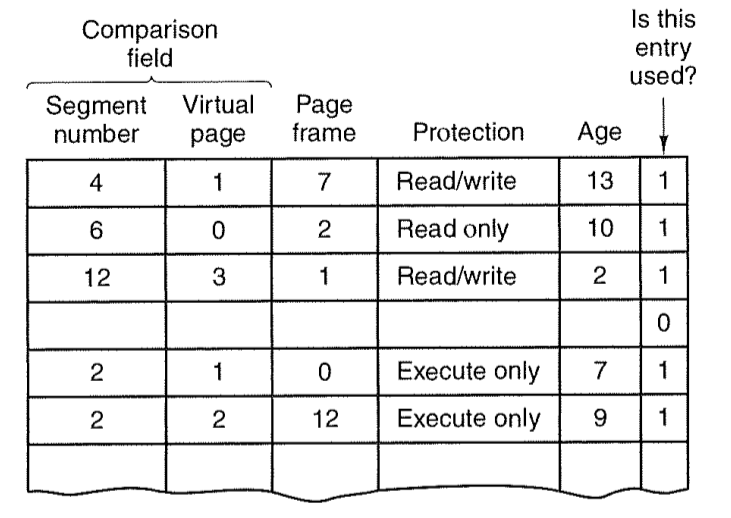
\includegraphics[width=1.0\textwidth]{tlb2.png}

思考:最后两列的用途
\end{frame}

\begin{frame}{Intel平台上的分段分页技术: GDT与LDT}
Intel平台上,所有段表分成两类:
\begin{enumerate}
\item[]
\item GDT (Global Descriptor Table) -- 系统段(OS), 仅1个
\item[]
\item LDT (Local Descriptor Table) -- 每个进程都有自己的LDT
\end{enumerate}
\end{frame}

\begin{frame}{Intel平台上的分段分页技术: 段选择符(Segment Selector)}
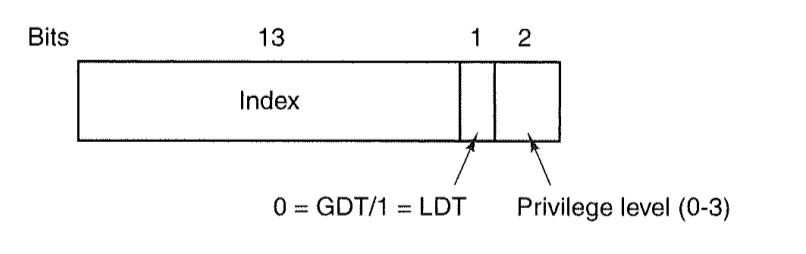
\includegraphics[width=1.0\textwidth]{selector.png}

\begin{description}
\item[CS寄存器] 存放代码段的段选择符
\item[DS寄存器] 存放数据段的段选择符
\item[其他] 四个段寄存器
\end{description}
\end{frame}

\begin{frame}{Intel平台上的分段分页技术: 段描述符(Segment Descriptor) -- 段表项}
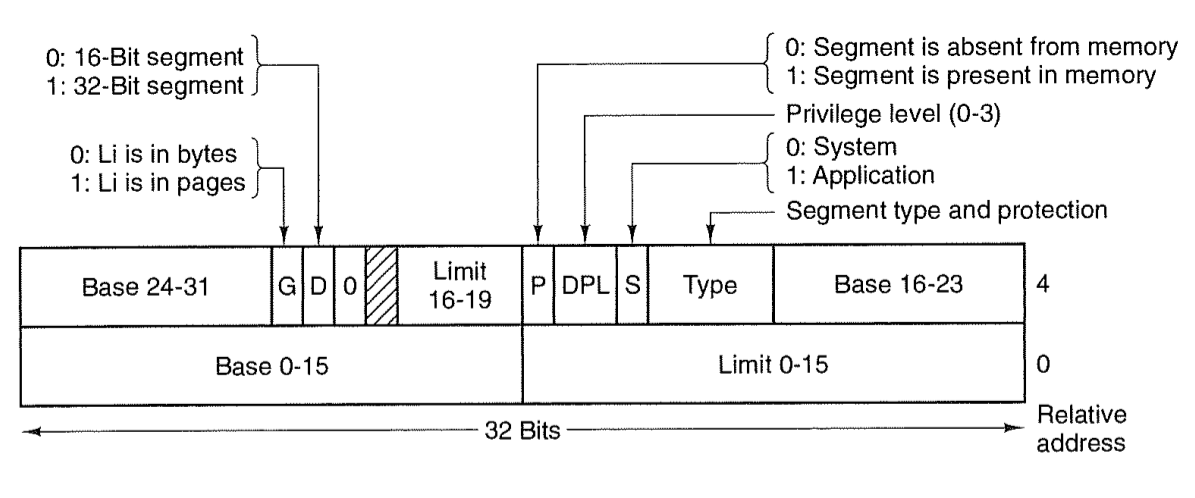
\includegraphics[width=1.0\textwidth]{descriptor.png}

三个关键字段:BASE,LIMIT,G
\end{frame}

\begin{frame}{Intel平台上的分段分页技术: 从(段选择符,偏移)到线性地址的映射}
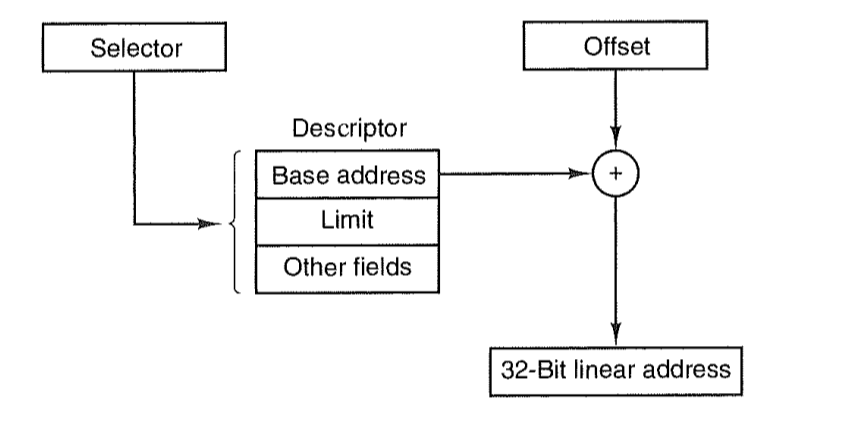
\includegraphics[width=1.0\textwidth]{smap.png}
\end{frame}

\begin{frame}{Intel平台上的分段分页技术: 从线性地址到物理地址的映射}
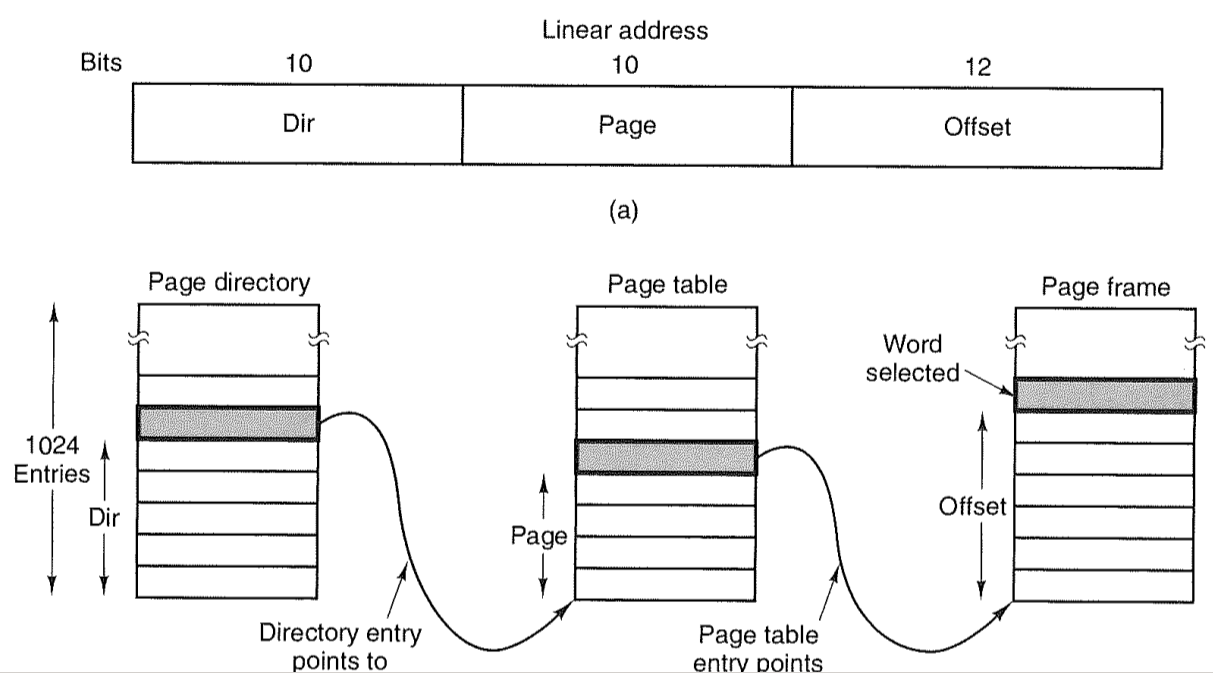
\includegraphics[width=1.0\textwidth]{pmap.png}
\end{frame}

\end{CJK*}
\end{document}
